\documentclass{standalone}
\usepackage{pgfplots}
\pgfplotsset{compat=newest}

\begin{document}
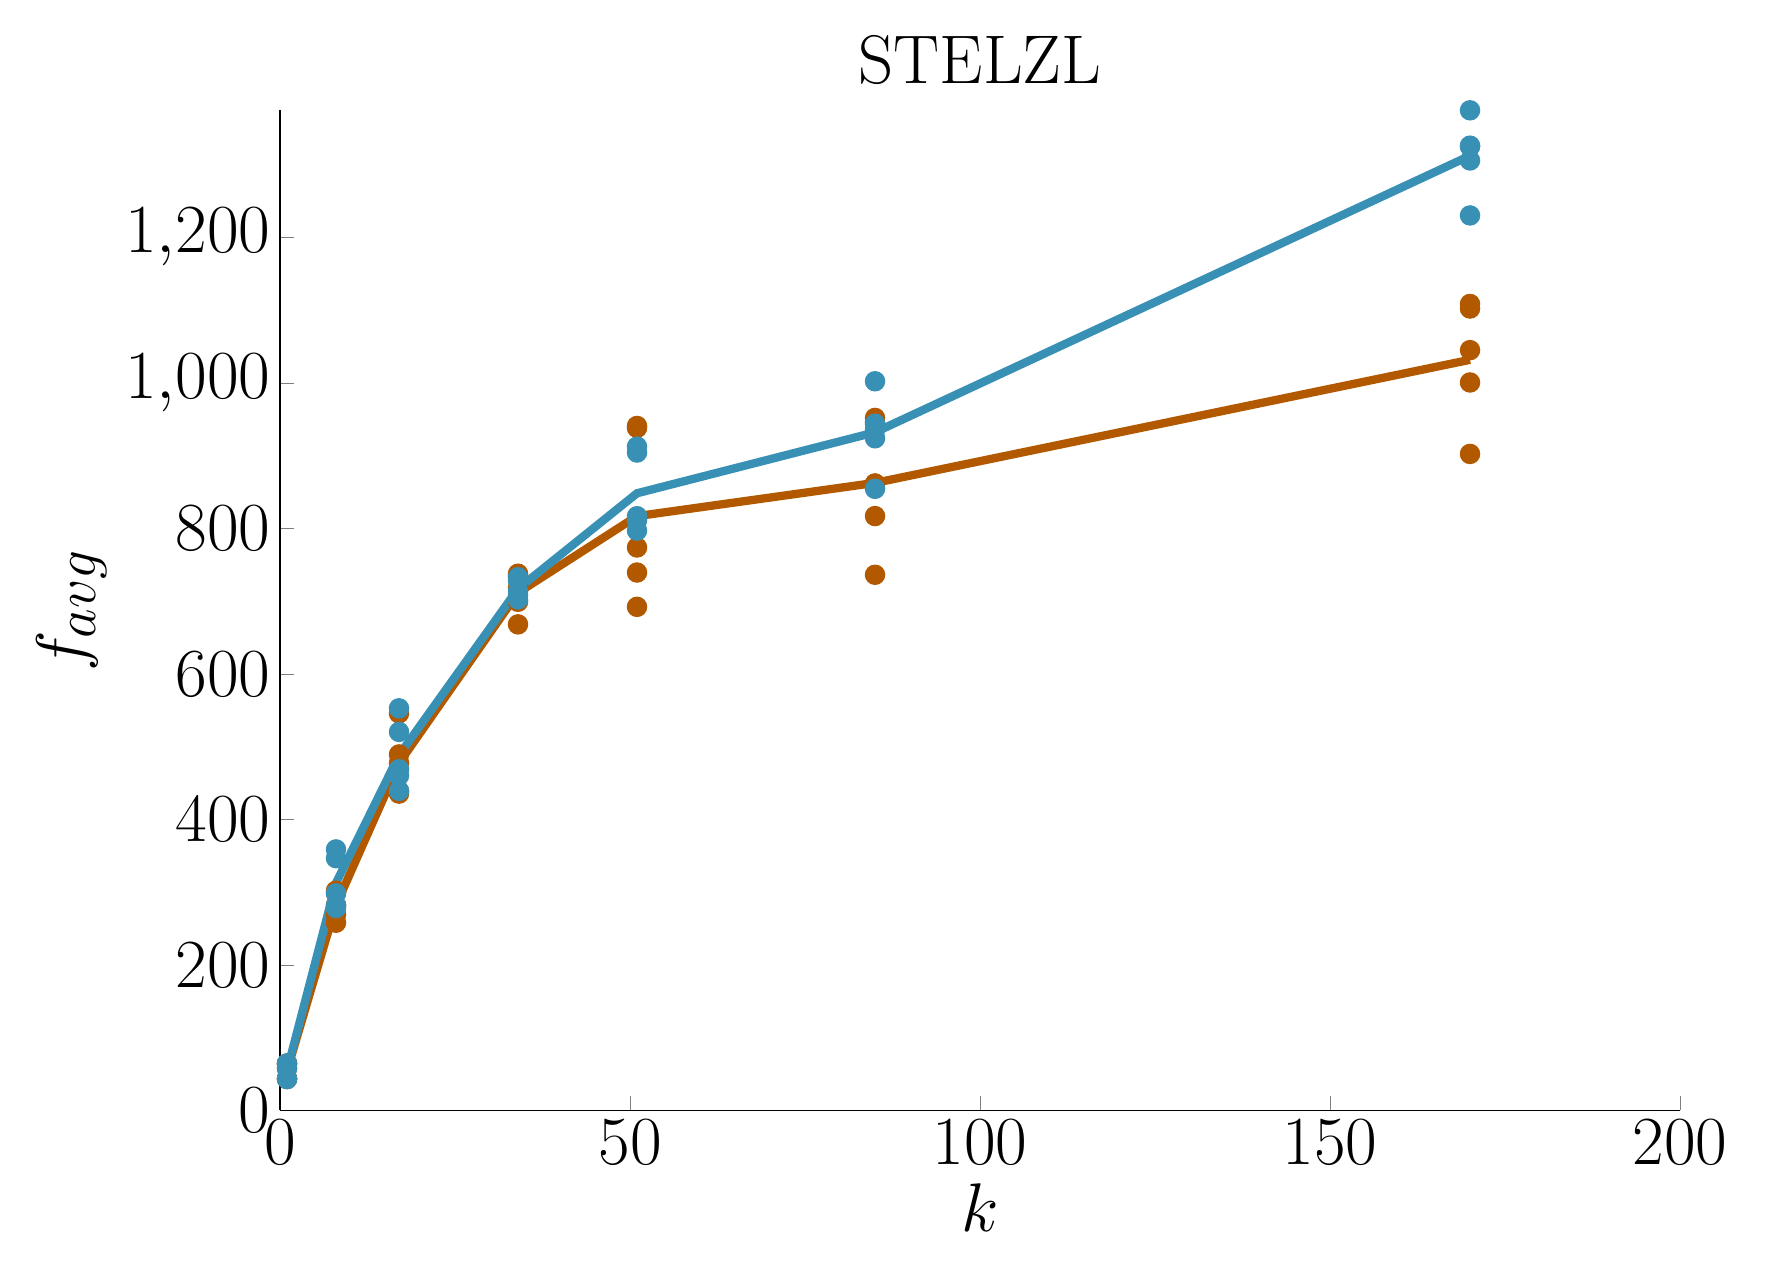
\begin{tikzpicture}

\begin{axis}[%
title style={font=\Huge},
title=STELZL,
tick label style={font=\Huge},
label style={font=\Huge},
legend style={font=\Huge},
view={0}{90},
max space between ticks=50pt,
width=7in,
height=5in,
scale only axis,
xmin=0, xmax=200,
xtick={0, 50, 100, 150, 200},
xlabel={$k$},
ymin=0, ymax=1374.75,
%ytick={0, 200, 400, 600, 800, 1000},
ylabel={$f_{avg}$},
major tick length=5pt,
axis lines*=left,
legend cell align=left,
clip=false]

\addplot [
only marks,
mark=*,
mark size=3.5pt,
color=orange!70!black,
%solid,
%line width=2pt,
]
coordinates{
(1,42.95)(1,43.45)(1,57.75)(1,64.2)(1,64.25)(8,257.9)(8,269.1)(8,281.95)(8,299.1)(8,301.9)(17,435.4)(17,438.8)(17,477.5)(17,489.25)(17,545.65)(34,668.05)(34,699.1)(34,718.15)(34,735.05)(34,737.7)(51,692.15)(51,739.3)(51,773.75)(51,938.15)(51,940.8)(85,736.25)(85,816.95)(85,861.85)(85,945.8)(85,951.85)(170,902.35)(170,1000.6)(170,1045.05)(170,1102.25)(170,1108.5)
};

\addplot [
only marks,
mark=*,
mark size=3.5pt,
color=cyan!70!black,
%solid,
%line width=2pt,
]
coordinates{
(1,42.95)(1,43.45)(1,57.75)(1,64.2)(1,64.25)(8,278.1)(8,281.55)(8,298.25)(8,346.65)(8,358.65)(17,439.15)(17,460.05)(17,468.85)(17,520.2)(17,552.65)(34,702.4)(34,708.3)(34,713.15)(34,727.85)(34,732.8)(51,796.9)(51,811.05)(51,816.7)(51,904.3)(51,912.45)(85,854.4)(85,923.9)(85,935.85)(85,943.9)(85,1002.25)(170,1230.2)(170,1305.8)(170,1324.85)(170,1326.15)(170,1374.75)
};

\addplot [
color=orange!70!black,
solid,
line width=3pt
]
coordinates{
(1,54.52)(8,281.99)(17,477.32)(34,711.61)(51,816.83)(85,862.54)(170,1031.75)
};

\addplot [
color=cyan!70!black,
solid,
line width=3pt
]
coordinates{
(1,54.52)(8,312.64)(17,488.18)(34,716.9)(51,848.28)(85,932.06)(170,1312.35)
};


\end{axis}
\end{tikzpicture}
\end{document}
